\subsubsection{Sistema de ventilación}

Para este sistema, se ha propuesto utilizar dos ventiladores de computadoras, uno de ellos cumplirá la función de introducir aire al interior del contenedor, buscando en primera instancia, reducir la temperatura al interior del tambo, en caso de que esta se encuentre por arriba de los parámetros deseados, y al mismo tiempo permita airear la mezcla de residuos al interior del contenedor.

La función del segundo ventilador será la de facilitar la salida del aire desde el interior hacia el filtro encargado de eliminar los olores.
\\
\begin{figure}[h!]
            \centering
            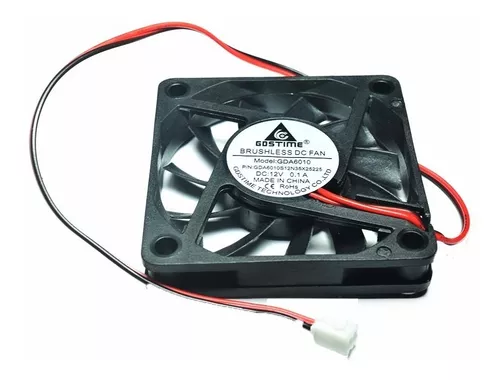
\includegraphics[scale=0.5]{images/Capitulo 4/s5/Contenedor/ventilador.png}
            \caption{Ventilador propuesto para el sistema de ventilación}
            \label{fg:ventilador}
     \end{figure} \newpage


\begin{table}[h!]
    \centering
    \caption{Características del ventilador}
       \begin{tabular}{|c|c|}
\hline
Dimensiones & 60mm x 60mm x 10mm \\
\hline
Tipo de conector & Dos pines \\
\hline
Alimentación & 12V \\
\hline
Consumo de corriente & 0.1A \\
\hline
Velocidad & 3500 rpm \\
\hline
Flujo de Aire & 21.5 cfm \\
\hline
Peso & 25 gramos \\
\hline
Longitud del cable & 25cm \\
\hline

\end{tabular}
    \label{tab:ventilador}%
\end{table}

Se realizaron algunas simulaciones con distintas distribuciones de los ventiladores, con el propósito de observar su comportamiento y elegir la más adecuada buscando que una vez inyectado el aire al interior del contenedor, este se distribuya de manera uniforme por otro lado, se requiere que su manufacturasea sencilla, pues pondría en riesgo una de los elementos más importantes como lo es el tambo.
La opción que mejores resultados dio tomando en cuenta lo previamente mencionado se presenta a continuación:
\begin{figure}[h!]
            \centering
            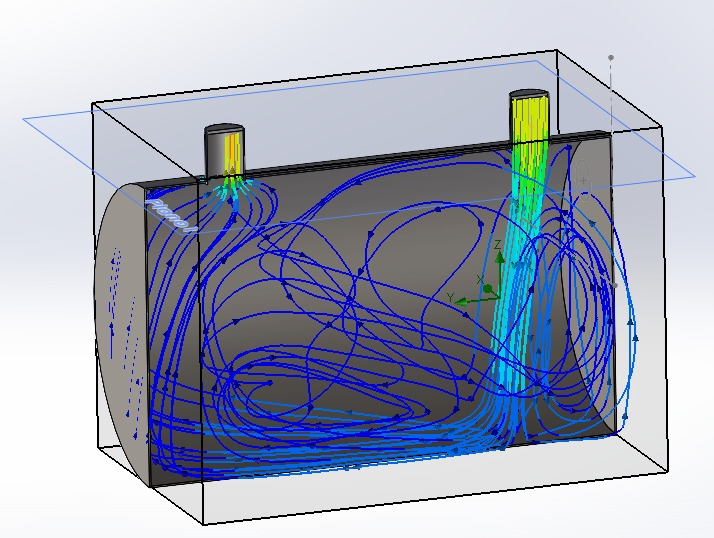
\includegraphics[scale=0.4]{images/Capitulo 4/s5/Contenedor/Est_Termicos/ventilacion_ultima.jpg}
            \caption{Configuración de ventiladores, aire inyectado entrada del triturador }
            \label{fg:ventilador_cilindro}
     \end{figure}
 
 \newpage